\section{Analytical Modeling Of MPI Applications}
\label{sec-model}

To effectively reduce the overhead of network communications in MPI applications,
one must understand when and where it becomes beneficial to enhance the overlap of communications with local computations in these applications,
In particular, through an analytical approach, our framework aims to model the runtime execution flows of an input application in terms of their relative amount of time spent in local computations and network communications.
This information then is used to automatically identify potential communication bottlenecks as candidates for optimization in the later steps.

The purpose of our execution flow modeling is to estimate the time required to complete each MPI communication in relation to adjacent computations on the local node.
To represent runtime execution paths and estimate the time required to execute the local computation of each path, we use the  \texttt{Bayesian Execution Tree} (\texttt{BET})  from the Skope analytical performance modeling framework~\cite{jichi:ipdps14}.
Each BET essentially represents possible runtime code paths of an application together with their execution frequency and expected execution time. We use the Skope framework to automatically generate a BET representation of each application from the application source code combined with some sample input data and code-coverage  profiling of the application execution.
We then extend the Skope framework to additionally estimate the overhead of each MPI communication through the following steps.
\begin{enumerate}
\item Use LogGP-based communication model for the MPI runtime to estimate the communication time for each individual MPI call.
\item Statistically estimate the expected average communication time for each code path by combining the individual communication with the execution frequencies.
\end{enumerate}
The balance between the time required for each MPI communication and the expected execution time of its surrounding local computation is used to project optimization opportunities. The following first illustrates the BET representation that we inherit from~\cite{jichi:ipdps14} and then explains our extensions for modeling MPI communications.

\subsection {Bayesian Execution Tree}

\begin{figure}[h]
\begin{center}
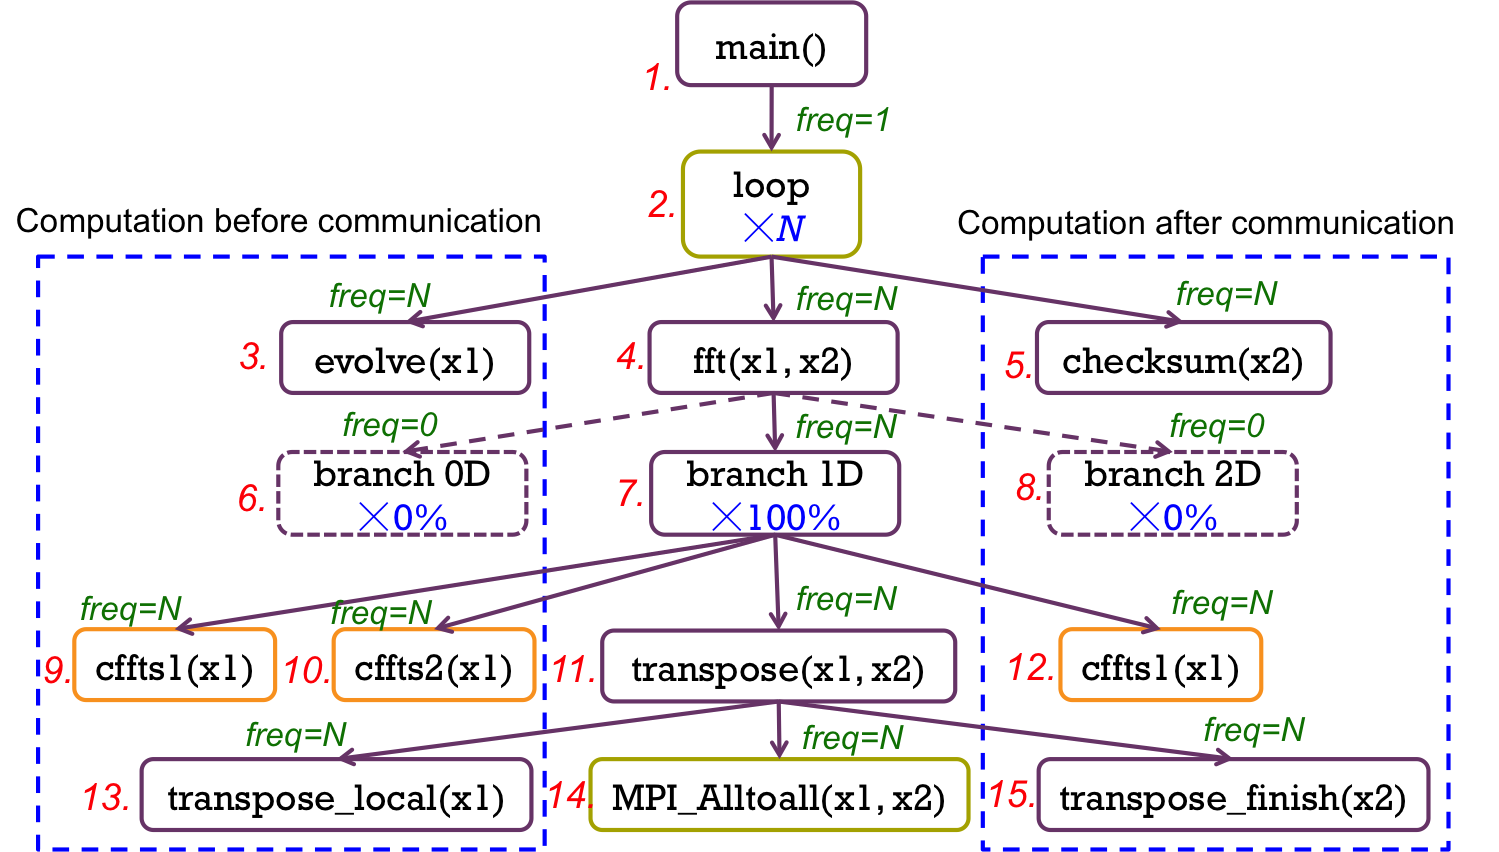
\includegraphics[width=0.48\textwidth]{fig/ft_bet.png}
\caption{Simplified Bayesian Execution Tree for NAS 1D FFT before overlapping computation and communications
  \emph{(for simplicity, only important branches, loops, and function calls are shown, and not all nodes and frequencies in BET are drawn in this figure)}
}
\label{fig:ft_bet}
\end{center}
\end{figure}

Figure~\ref{fig:ft_bet} shows an example \texttt{BET} for one of the MPI processes of the 1D FFT benchmark in Figure~\ref{fig:ft_loop}.
Each node of the BET represents a code block (a sequence of statements in the user program) together with its runtime \emph{execution frequency}, defined as the expected average number of times that statements in the node block will be executed at runtime.
A \texttt{depth-first-traversal} (\texttt{DFS}) of each subtree of the \texttt{BET} corresponds to a possible runtime execution path of the statements.
For example, in Figure~\ref{fig:ft_bet}, Node\#2 is a loop of $N$ iterations, so the frequency of its loop body is $N$.
Node\#7 is a branch inside {\em fft} function. If the application is to perform 1D FFT,  this branch is taken 100\% of time during execution,
so its frequency is $N$, while the frequency of the alternative branches (Node\#6 and Node\^8) are set to 0.


In order to derive execution frequencies of each code block, the Skope framework requires a description of the application input data,
either manually provided by the user or automatically collected via an instrumented run of the application.
The input data description characterizes the possible values of all the data that the application may obtain from external sources,
for example, command-line arguments, environment variables, or files.
For array variables, only their dimensions and the size of dimension are required.
For MPI applications, the total number of MPI processes (\texttt{MPI\_Comm\_size}) and the rank of the process to model (\texttt{MPI\_Rank}) are additionally required.
Based on the input data description, the Skope framework applies constant propagation to derive possible values of the expressions that
control the directions of branch and loop controls. A fall-through probability to be 50\% is assumed if the values cannot be accurately determined.
% and function arguments from source code into \texttt{BET}. %through data dependence analysis.
%Given the input data description, we then evaluate these expressions through a depth-first-traversal of \texttt{BET}
%  in a process that is similar to \emph{Constant Propagation}.
%To reduce the overall evaluation time,
%  the evaluations that involve arrays are skipped.
%As the result, plus there could be unspecified values for the input array data,
%  not all branch conditions and loop controls be accurately computed.
%Take if-branch as an example.
%To further improve the accuracy of the execution frequencies,
%  users can also provide the code coverage profiling data.
For this paper, we used \texttt{gcov} to profile applications with sample input data,
%Finally, after knowing the values or probabilities of branch conditions and loop controls,
%  the execution frequency for each node is computed through a top-down traversal of \texttt{BET}.
%In particular:
%\begin{itemize}
%\item For a code block that is neither a branch nor a loop, its execution frequency is the same as that of its parent.
%\item For a branch, its execution frequency is its fall-through probability multiplying by its parent node's execution frequency.
%\item For a loop without breaks, its execution frequency is the number of iterations multiplying by its parent node's execution frequency.
%\item For a loop with $N$ iterations in the loop control while having a break in a branch whose fall-through probability is $P_{break}$, then
%    its execution frequency equal to its parent node's execution frequency multiplying by the following equation:
%\begin{equation}
%  Freq(N,P_{break}) = \frac{1 - (1 - P_{break})^N}{P_{break}}
%\end{equation}
%\end{itemize}


\subsection{Modeling MPI Communications}

To predict how to better overlap MPI communications with local computations, we have extended the Skope framework
with the LogGP model~\cite{loggp} to additionally model the latency (elapsed time) of each MPI operation using the following four parameters:
  \begin{enumerate}
  \item $P$: number of processes involved in the communication %in $mpi\_op$,
  \item $n$: size (in bytes)of the message being transferred 
  \item $alpha$: overhead of starting each message and time interval required between transmitting each pair of messages
  \item $beta$:  expected communication time per byte for large messages,  determined by the underlying network bandwidth.
\end{enumerate}
Among the four parameters, $alpha$ and $beta$ can be calculated from characteristics of the underlying network.
In particular, we compute $beta$ as the reciprocal of the network bandwidth  and $alpha$ by using microbenchmarks to measure the latency of \texttt{MPI\_Send} and \texttt{MPI\_Recv} operations on the target platform.
The other two parameters,  $P$ and $n$, are either determined through instrumented runs of the user application or obtained directly from the user as expected runtime configurations of the application.
 In particular, $P$ equals to \texttt{MPI\_Comm\_size};  and $n$ (i.e., message size) is obtained from the values used to invoke the MPI operations.

Following the LogGP model, we model MPI point-to-point communications as
\begin{equation}
cost_{p2p}(n;alpha,beta) = alpha + n\cdot beta .
\end{equation}
To model the \texttt{MPI\_Alltoal} operation,  we use the following two formulas.
\begin{equation}
  cost_{short} = log P\cdot alpha + \frac{n}{2}\cdot log P\cdot beta
\end{equation}
\begin{equation}
cost_{long} = (P-1)\cdot alpha + n\cdot beta
\end{equation}
The first formula models the communication time of short messages and the second that of long messages.
We use values of \emph{control variables} from  the MPI runtime library, for example, \texttt{MPIR\_CVAR\_ALLTOALL\_SHORT\_MSG\_SIZE} for MPI alltoall,
%  which can be obtained by running \texttt{mpivars} on the target platform.
to determine whether a message should be categorized as {\em short} or {\em long} and thereby select the proper formulas to use.

%LogGP models each communication through the use of five parameters:
%  maximum communication latency ($L$),
%  overhead ($o$),
%  gap between messages ($g$),
%  gap per byte for long messages ($G$),
%  and the number of processors ($P$).
%Because the MPI standard does not enforce the communication algorithm to implement MPI API,
%  the formula of communication cost could be different for different MPI runtime library.
%Given the LogGP communication model~\cite{loggp}, the communication time of MPI operations can be estimated
%  from the message sizes, topology of the processes, network bandwidth and latencies.
%In our framework, we adopt the modeling formulas that we found in the source code of MPICH 3.1~\cite{mpich2}.
%In general, and we model the communication cost for MPI operation $f$ as follows:



%{\scriptsize
%\begin{verbatim}
%int MPI_Alltoall(
%  const void *sendbuf, int sendcount, MPI_Datatype sendtype,
%  void *recvbuf, int recvcount, MPI_Datatype recvtype,
%  MPI_Comm comm)
%\end{verbatim}
%}%\scriptsize

%It has different cost formulations for small and large messages respectively.
%The threshold message size could be found by executing \texttt{mpivars} on the target cluster.

%LogGP models collective MPI communications by using \todo {summarize the approach}.
%Given the LogGP models, the collective MPI communications cost can be modeled theoriodically given the algorithm of the MPI operation.
%Since the MPI standard does not always specify the algorithm to implement each MPI function,
%  the cost formula are usually implementation-dependent for different MPI runtime library being used.
%In our approach,
%  we used MPICH 3.1~\cite{mpich2} as the runtime library in the experiment,
%  and the cost formula we found in MPICH's source code are used to model the communication cost in our approach.
%For example, we modeled MPI alltoall, broadcast, and reduce, and allreduce operations by using the following equations.

After estimating the execution time of each individual MPI operation,
  the overall communication time of a code path in BET can be calculated by adding the communication time of all code blocks along the path, using the following formula.
\begin{equation}
  cost_{n} = \sum\limits_{i}^{n} cost(i) * freq(i)
\end{equation}
Specifically, the total communication cost of a path of $n$ nodes in the BET can be computed as the sum of
  the communication time of each individual MPI operation multiplied by its execution frequency $freq(i)$.
Here, $freq(i)$ is calculated by using BET as one of the properties of the BET node that contains the MPI operation,
and $cost(i)$ is calculated as indicated above using LogGP formulas instantiated with the expected parameter values of the MPI operations.
For example, the total communication time of \texttt{MPI\_Alltoall} in Figure~\ref{fig:ft_bet} can be computed by
  multiplying the average communication time of \texttt{MPI\_Alltoall} by the number of iterations of the loop node\#2 ($\times N$)
  and the fall-through probability of the 1D FFT branch node\#7 ($\times 100\%$).

% EOF

%To estimate the execution time of individual MPI operation,
%  we use the LogGP communication model~\cite{loggp} that is an extension of the LogP communication model~\cite{logp}.
%The LogGP communication model~\cite{loggp} is widely used to estimate communication cost for distributed computation.
%It is an extension of the LogP model~\cite{logp} that
%  abstracts the communication process of short messages using four parameters:
%  communication latency (\texttt{L}),
%  overhead (\texttt{o}),
%  bandwidth (\texttt{g}),
%  and number of processors (\texttt{P}) involved in the communication.
%And the LogGP model extends the LogP model to support long messages
%  by adding an additional parameter that captures the bandwidth obtained for the long messages (\texttt{G}).
%Given LogGP model, the communication cost of MPI operations
%  can be modeled from the number of processes, network latencies of the hardware, and the communication algorithm of the implementation.
%For example, the cost of point-to-point communication using \texttt{MPI\_Send} and \texttt{MPI\_Recv} can be computed as follows:
%% through the use of five parameters:
%%  maximum communication latency ($L$),
%%  overhead ($o$),
%%  gap between messages ($g$),
%%  gap per byte for long messages ($G$),
%%  and the number of processors ($P$).
%\begin{equation}
%cost(n;alpha,beta) = alpha + n\cdot beta
%\end{equation}
%Where
%$alpha$ is the startup cost per message (corresponding to \texttt{L} and \texttt{o}),
%$n$ is the message size in bytes,
%and $beta$ is the reciprocal of bandwidth, i.e. cost per byte for long messages (corresponding to \texttt{G}).
%% On BG/Q, $alpha$ and $beta$ might be different for short/long message.
%However, this formula does not consider the wait time spent among the unbalanced processes,
%  which is runtime-dependent on the time when the two processes start communication.
%%If the MPI processes are not well balanced,
%When the send and receive operations are not well balanced at runtime,
%  it may under-estimate the overall time spent to complete the entire communication.

%\done{jichi: The following paragraph is the last version of the text that I think we could delete}
%
%Then, we modify the Skope framework to additionally  estimate overhead of MPI communications through the following extensions.
%
%\todo {rewrite the following to be extensions to the Scope summary}
%\begin{enumerate}
%\item Parameters of global MPI runtime configuration such as the communicator size and process rank are predefined by developers as part of the input data,
%  which will be used to compute return values of \texttt{MPI\_Comm\_size} and \texttt{MPI\_Rank}.
%\item MPI calls are preserved in the execution paths,
%  and the runtime values of their \emph{scalar} arguments on each execution paths are computed
%  through either constant propagation from the input data,
%  or runtime profiling of the function calls.
%\item The communication time for each MPI function call %on each code path
%    is projected from its runtime arguments and global MPI configuration using the formula of the underlying MPI runtime library derived from LogGP communication model.
%\item The execution frequency of each MPI call are computed,
%  and the communication time of the MPI operation on each code path are aggregated from the communication time of all MPI calls on the code path and their execution frequencies.
%  %We construct an intermediate representation, a Bayesian Execution Tree (BET),  of the execution flow model of the MPI's application master process (rank 0),
%  %and then, analytical performance models are used to estimate communication and computation time of each node in BET.
%\end{enumerate}
%
%This extended Scope framework produces a representation the runtime execution paths of the application,
%\todo { expand to be more precise, maybe have an example output, and explain precisely what the output is}
%  with the computation and communication time on each portion of the execution paths are projected.
%\todo {explain the following using an example}
%\todo { Summarize the key technical challenges of the above extensions and the key sollutions. The organize
%the rest into three subsections, one describing the extended BET with an example, and the other explaining the
%MPI modeling details}
%
%
%In particular, the execution paths are represented by a Bayesian Execution Tree structure (\texttt{BET}) in the Skope framework.
%Each node in \texttt{BET} is associated with a code block or instruction in source code,
%  and the parent of a node is associated with most enclosing parent code block of that node.
%As the word \textit{Bayesian} indicated, each node also has a property of execution frequency.
%The code path starting at each node could be represented by a depth-first traversal from that node
%  with MPI function calls and computation instructions in the nodes on the code paths.
%Such \texttt{BET} structure will be used to help make the overlap optimization profitable later.
%
%The following paragraphs will discuss each of the extra steps to model MPI applications in details.
%
%\subsection{MPI configuration parameters}
%In our current Skope framework, a BET is constructed for each process.
%And we use constant propagation to compute most properties of BET from input data.
%Because the number of MPI processes and the rank of a process are determined at runtime,
%  the return values of \texttt{MPI\_Common\_size} and \texttt{MPI\_Rank} are unknown offline.
%It will cause the values of many variables unable to be computed offline and hence reduce the accuracy of the modeling of the execution paths.
%Currently, we need use users to manually specify the runtime values of MPI communicator size and rank,
%  and the modeling and optimization later will then be based on this specific configuration.
%
%\subsection{Calculating function parameters}
%\todo { this seems out-of-order. Why isn't this part of the LogGP model section? Is this part of the key steps/tasks?}
%
%In order to estimate runtime for each individual MPI function,
%  the runtime values of the function call are indispensable.
%In our approach, the MPI communication modeled in our approach include
%  send/receive, alltoall, broadcast, reduce, and allreduce.
%The parameters needed to be modeled such as the message sizes are usually saved in scalar variables.
%Using BET, the runtime values of a large amount of scalar variables can be calculated offline
%  given the input data of the application.
%If a MPI function parameter can not be computed offline through constant propagation from the given input data,
%  it is needed to be provided by the developers through domain knowledge or profiling at runtime. %from runtime hints.
%
%
%An MPI communication model needs to be constructed and combined with local dataflow analysis that estimates the runtime parameters of MPI calls and the control flow paths leading to the calls.
%The runtime parameters such as the message types and sizes will be used to calculate the time for an individual communication operation,
%  and the control flow paths are needed to estimate the total number and probabilities of the communication operation that will be executed.
%\todo {summarize the technical approach. Explain BET and cite previous work as appropriate. Remove any detail from the previous paper that is irrelevant to the new paper, rewrite to focus topics related to this paper!}
%\done{
%In our approach, we adopt an analytical execution flow modeling approach
% to extract and summarize the runtime code paths of the application out of its source code,
% which is needed to calculate runtime parameters to invoke individual computation and communication loops and functions,
% and how frequently these basic computation and communication will be executed.
%In particular, we will construct a Bayesian Execution Tree (BET) for each MPI process with specific rank.
%The BET is a tree structure
%  with node representing an instruction or code block in the source code,
%  and the parent of a node is associated with most enclosing parent code block of that node.
%The properties of each node
%  might not contain all the instruction(s) that will be executed,
%  but only the performance impact of these instructions,
%  their execution frequency (number of execution or propability of the execution),
%  and the expressions that how scalar variables that are being modified after executing this node.
%
%The performance includes the computation intensity (represented by the numbers of integer and floating-point instructions)
%  and memory side effects (represented by memory loads and stores).
%Combined with Roofline model, also given the specification of the target hardware,
%  these information can be used to estimate the upper-bound of the computation time that are needed to evaluate instructions in this node for 1 time.
%
%The execution frequency represents the probability of the total number of execution times for a node.
%For example, given a for-loop, it's frequency of it's body block will be the number of iterations that the loop will be executed.
%If this for-loop is in the true-branch of a if-branch, then its frequency will also multiple by the fall-through probability of the true code path.
%Instead, if this loop is in an unreachable branch of a if-branch, then its frequency will be zero.
%And if there are break/continue in the for-loop, given the probability the continue/break will happen, the expectation of the loop iteration count will be calculated and used as the execution frequency of this loop.
%
%Beyond performance impact and execution frequency, each node in BET also holds
%  the expression that certain variable are being computed.
%These expressions are needed so that certain important variables such like the loop count and function parameters can be computed offline.
%Note all instructions are being kept in the BET node.
%Only instructions that are needed to compute critical scalar variables are preserved,
%  which include the scalar variables used as function parameters, loop count, if/switch condition,
%  and all other intermediate variables that the computation of critical variables depends on.
%The values of intermediate arrays used in the computation are not tracked for better evaluation speed.
%
%The Bayesian Execution Tree (BET) of a MPI application is not constructed in one-pass.
%In our approach, our first-pass extracts a BET with performance impact and scalar variable expressions only from the application's source code
%  leaving execution frequency empty.
%Then, the second-pass combines constant propagation with user-specific input data and code coverage profiling results
%  to calculate the execution frequency for each node in BET.
%We divide the BET construction into two passes,
%  because the first pass is mainly based on static program analysis,
%  while the second pass integrating with the domain knowledge about the input data and application's runtime behavior from developers and/or from profiling.
%}%\done

%To quickly gain first-order insights about hot regions and reasons behind their performance bottlenecks,
%  we have designed a framework to analytical model the holistic execution flow of a sequential application
%  and then employ parameterized hardware performance models to project application performance for varying architecture design configurations.

%We design a Bayesian Execution Tree (BET) representation of the execution flow
%  to express the runtime code path and performance characteristics along the path,
%    including the numbers of estimated instruction counts and memory accesses.
%A Bayesian execution tree is first constructed from the application's source code, input data, and input-dependent code coverage profiling results.
%And then, the execution time for each code path in BET is estimated using the Roofline model~\cite{roofline}.
%Our approach essentially uses statistical execution flow models of applications and coarse-grained performance models of hardware to project application performance on a prospective architecture without requiring any simulation or instrumented execution of the application on the target hardware.
%Local profiling is needed only once to gather the branch frequency statistics,
%  and the profiling results can be reused to analyze and project performance across different architectures.
%By mathematically modeling the repetitive control flow caused by looping,
%  the analysis and projection time does not scale with the input data size or the actual execution time of the application.
%By modeling the application execution flow, we are able to gain “contextual” insights such as the control flow leading to individual hot spots,
%  the relations among hot spots,
%  and sizes of input data associated with each invocation of a hot spot.
%Moreover, we can project whether computation or memory access is the bottleneck.

%To model the execution flow of MPI applications, we have extended the sequential execution flow model in \todo {cite previous paper}
%to additionally \todo {explain the following better, in terms of the extensions needed and what is exactly done} the runtime number of total processes and the rank of the process to model are needed to be specified by the developers.
%%One BET will be constructed for single MPI process with specific rank.
%%In my current approach, the BET of the the master process whose rank is 0
%%  is used to identify potential performance bottlenecks.
%In particular, the return values of \texttt{MPI\_Comm\_size()} and \texttt{MPI\_Comm\_rank()} are specified while constructing BET.
%Additionally, all MPI calls are preserved in the BET as opaque function calls instead
%  of being replaced by the estimated performance characteristics.

% Our previous work
% 1. Code skeleton semantics and generation -- ignored as we didn't change the skeletons in order to support MPI
% 2. Execution flow modeling using BET
% 3. Performance projection and hot spot analysis

%The framework presented in this paper extends
%  our previous analytical modeling work for identifying potential hot spots in sequential applications~\cite{jichi:ipdps14}.
%In this paper,
%  we extend our SKOPE framework for modeling sequential applications~\cite{jichi:ipdps14}
%  to support modeling MPI communication.
%We extend our application model %in the SKOPE
%    %to be aware  of MPI function calls,
%    to be able to capture the MPI function calls and the runtime parameter values,
%  and extend the performance projection
%    to use the LogGP communication model~\cite{loggp} to estimate the communication cost of these functions.
%The following sections will summarize
%  the related approaches in the SKOPE for modeling computation in sequential workflow,
%  and the LogGP communication model. %we used.

%\subsubsection{Code skeletons}

%The performance projection takes three steps:
%\begin{enumerate}
%\item The message size arguments for MPI function calls are computed by evaluating BET.
%\item Communication cost is estimated for each MPI function from
%    the computed message sizes, user-specified number of processes, and the type of the MPI function.
%\item The communication cost for the BET node of each MPI function calls
%    are is estimated by the communication cost of the function multiplying by the execution frequency of the node.
%\end{enumerate}

% Blocking VS Non-blocking and Wait time
%Our current modeled MPI functions include MPI \texttt{send}, \texttt{receive}, \texttt{alltoall}, \texttt{broadcast} and \texttt{reduce}.
%The communication cost for both blocking or non-blocking communication is estimated in the same way using the LogGP model.
%Currently, because we didn't model the interactions among processes,
%  we could not model the wait time of \texttt{MPI\_Wait} and \texttt{MPI\_Waitall}
%  whose communication cost is ignored.

%For each point-to-point or collective MPI communication function call in the BETs,
%we first compute its runtime arguments at the call site %, and use the LogGP model to estimate the communication cost.
%that usually include %the array buffer to send or receive,
%the number of elements to send or receive and the element data type, %, and the ranks of sender of receivers.
%which could be used to compute the total number of bytes to communicate.
%Then, combining with the MPI communicator size from the runtime hints,
%the LogGP model is able to estimate the communication cost for this call.
%Currently, we didn't consider the sub-communicator.

%Our technique is built upon previously proposed modeling techniques.
%The overall workflow of our framework is shown in Figure~\ref{fig:overview}.
%It takes the application's source code as well as the profiling results and hardware models,
%and generates the source code optimized for the target runtime environment.
%The workflow that can be divided into the following four stages:
%%\begin{enumerate}
%%\item Hardware calibration to get the parameters for the computation and communication hardware performance models.
%%  The hardware performance models are used to analytically estimate computation and communication time for a workflow.
%%  The roofline model is used to model computation.
%%  And I developed a profiling-based communication model for estimating balanced MPI two-sided and collective communication time.
%%\item Skeleton-based modeling for course-grained analysis to find hot communication and candidate overlap code regions.
%%  First, an analytical execution-flow model will be constructed for the application.
%%  Then, combining with hardware models, the hot region analysis will be applied to find hot communication.
%%  %First, generate skeletons from the source code to construct an execution flow model.
%%  %Then, select a few top hot communication spots by the hot region analysis.
%%  And finally,
%%  an inter-procedural analysis will be applied on the execution-flow model
%%  to compute the candidate overlap region that might contain overlappable hot communication and computation.
%%\item Optimization analysis to compute overlappable computation in the estimated overlap code region.
%%  Given the hot communication and the enclosing overlap region,
%%  the optimization analysis will first apply annotation-based inlining to erase the procedure boundaries,
%%  and then
%%  %The first step is to use annotation-based inlining to help erase the procedure boundaries.
%%  use data dependence analysis and control flow analysis to find
%%  the computation that are either independent from the communication, or can be decomposed to interweave with the communication.
%%%\item Program transformation to generate the optimized code for the target hardware.
%%%  %Generating CCO pragmas
%%%  % Transform the code
%%\end{enumerate}
%%that can be divided into four stages, as follows:
%\begin{enumerate}
%\item Hardware calibration to get the parameters for the computation and communication hardware performance models.
%  The roofline model and LogGP model are used to model computation and communication respectively.
%  The roofline model parameters includes the peak CPU frequency, instruction cycles, memory latency and throughput, etc.
%  The LogGP model parameters are the communication latency per message and per byte. %, and the number of nodes at runtime.
%
%  %The hardware performance models are used to analytically estimate computation and communication time for a workflow.
%  %This thesis also develops a profiling-based communication model for estimating balanced MPI two-sided and collective communication time.
%\item Skeleton-based modeling to
%  construct an analytical execution-flow model for the application
%  and identify the communication and computation hot spots.
%  It is extended from the SKOPE framework~\cite{skope}
%  to model MPI applications.
%  The framework first automatically analyze the source code
%  and output \emph{code skeletons}, which summarizes the high level semantics that relate to performance behaviors of the underlying instructions.
%  We then build a model of the application's execution flow, a Bayesian execution tree (BET), from the code skeletons combining with code coverage profiling results.
%  Combining with the hardware performance models, the BET is used to identify the computation and communication hot spots.
%
%   %To model an input application,
%%We have extended %the {\em code skeleton} extraction component from the SKOPE framework~\cite{skope}
%%to automatically analyze the source code and abstract its performance behavior according to user-supplied input flags and data sets. %on varying architecture components.
%%The output is a {\em code skeleton} that summarizes the high
%%level semantics that relate to performance behaviors of the underlying instructions.
%
%  %We then build a model of the application execution flow to
%  % through local profiling based on a set of user-supplied input flags and data sets.
%  %The execution flow is then used to
%  %synthesize performance characteristics of each code block within the application.
%  %Finally, we use the roofline model~\cite{roofline} to estimate the performance of
%  %every code region, and the resulting execution flow model with performance
%  %estimations is used as input to identify hot spots and hot paths.
%  %Figure~\ref{fig:overview} summarizes our framework.
%
%  %First, an analytical execution-flow model will be constructed for the application.
%  %Then, combining with hardware models, the hot region analysis will be applied to find hot communication.
%  %First, generate skeletons from the source code to construct an execution flow model.
%  %Then, select a few top hot communication spots by the hot region analysis.
%  %And finally,
%  %an inter-procedural analysis will be applied on the execution-flow model
%  %to compute the candidate overlap region that might contain overlappable hot communication and computation.
%\item Optimization analysis to generate parameterized optimization pragmas
%  to overlap the hot communication and communication.
%  %to compute overlappable computation in the estimated overlap code region.
%  %Given the hot communication and the enclosing overlap region,
%  %the optimization analysis will first apply annotation-based inlining to erase the procedure boundaries,
%  %and then
%  %The first step is to use annotation-based inlining to help erase the procedure boundaries.
%  %use data dependence analysis and control flow analysis to find
%  %the computation that are either independent from the communication, or can be decomposed to interweave with the communication.
%\item Program transformation to generate the optimized code and tune for the target hardware.
%  %Generating CCO pragmas
%  % Transform the code
%\end{enumerate}
%
%In the following, we briefly introduce SKOPE's
%  code skeleton language,
%  Bayesian execution tree,
%  the Roofline and LogGP models.

%\IPDPS{
%\subsection{Code Skeletons}
%
%%Given an application, its code skeleton summarizes the
%%high level semantics that relate to performance behaviors of the underlying instructions.
%The code skeleton explicitly expresses all the control flows
%of the original code but replaces the actual instruction sequence
%with performance characteristics including iteration count,
%degree of parallelism, computation intensity, and data access patterns.
%A pedagogical example of the code skeleton language is shown in Figure~\ref{fig:bstbet}(a), which
%is structured similarly to its original source code in terms of
%functions, loops, branches, and data types.
%Two functions, {\em main} and {\em foo}, are declared in this example.
%
%% Review: Estimate manual efforts (#2,#4) and discuss input-dependency #2)
%% - Manual efforts are not mandatory, but could improve accuracy
%% - Profiling results are input dependent that can be done on different machines
%% - Mention the number of occurances of probabilities/loop counts in SORD
%% - Mention that the skeleton is input dependent
%%
%%\FIXME{jichi
%%Currently, the empirical estimations for run time dependent information is not fully automatized.
%%Skeleton generation will make placeholders for information unknown at compile-time.
%%The number of placeholders required for manual estimation is determined by how dynamic the application is rather than the scale of the application.
%%For example, we manually specified probabilities for 7 branches in the SORD (an earth quick simulation application written in Fortran) which contains 5000 lines of code.
%%Additionally, the information is input-dependent that can be retried by profiling the application on different hardware.
%%Automatic integrating profiling results is left for your future work.
%%}
%
%A code skeleton is parsed by SKOPE into a data structure
%named the {\em block skeleton tree} (BST). Figure~\ref{fig:bstbet}(b)
%shows the BST corresponding to the code skeleton in Figure~\ref{fig:bstbet}(a).
%Each node of the BST corresponds to a statement in the code skeleton.
%Statements such as function definitions, loops, or branches may
%encapsulate other statements, which in turn become the children nodes.
%%The BST is similar to the abstract syntax tree (AST) within a typical compiler
%%but with its nodes representing higher level run time statistics instead of
%%individual operations.
%% whose
%%leaf nodes can be individual operators and operands, the
%%BST representation works at a much higher level.
%%Figure~\ref{fig:bstbet}(b) illustrates the BST constructed from
%%the skeleton in Figure~\ref{fig:bstbet}(a).
%The BST does not contain information about the input.
%Consequently, it alone does not reflect the control flow and data flow,
%which are often input dependent.
%%affect the execution flow.
%%Consequently, both its control flow and data flow may vary significantly given different inputs, leading
%%to a wide variety of performance characteristics.
%}%\IPDPS
%
%\begin{figure*}[!htb]
%\begin{center}
%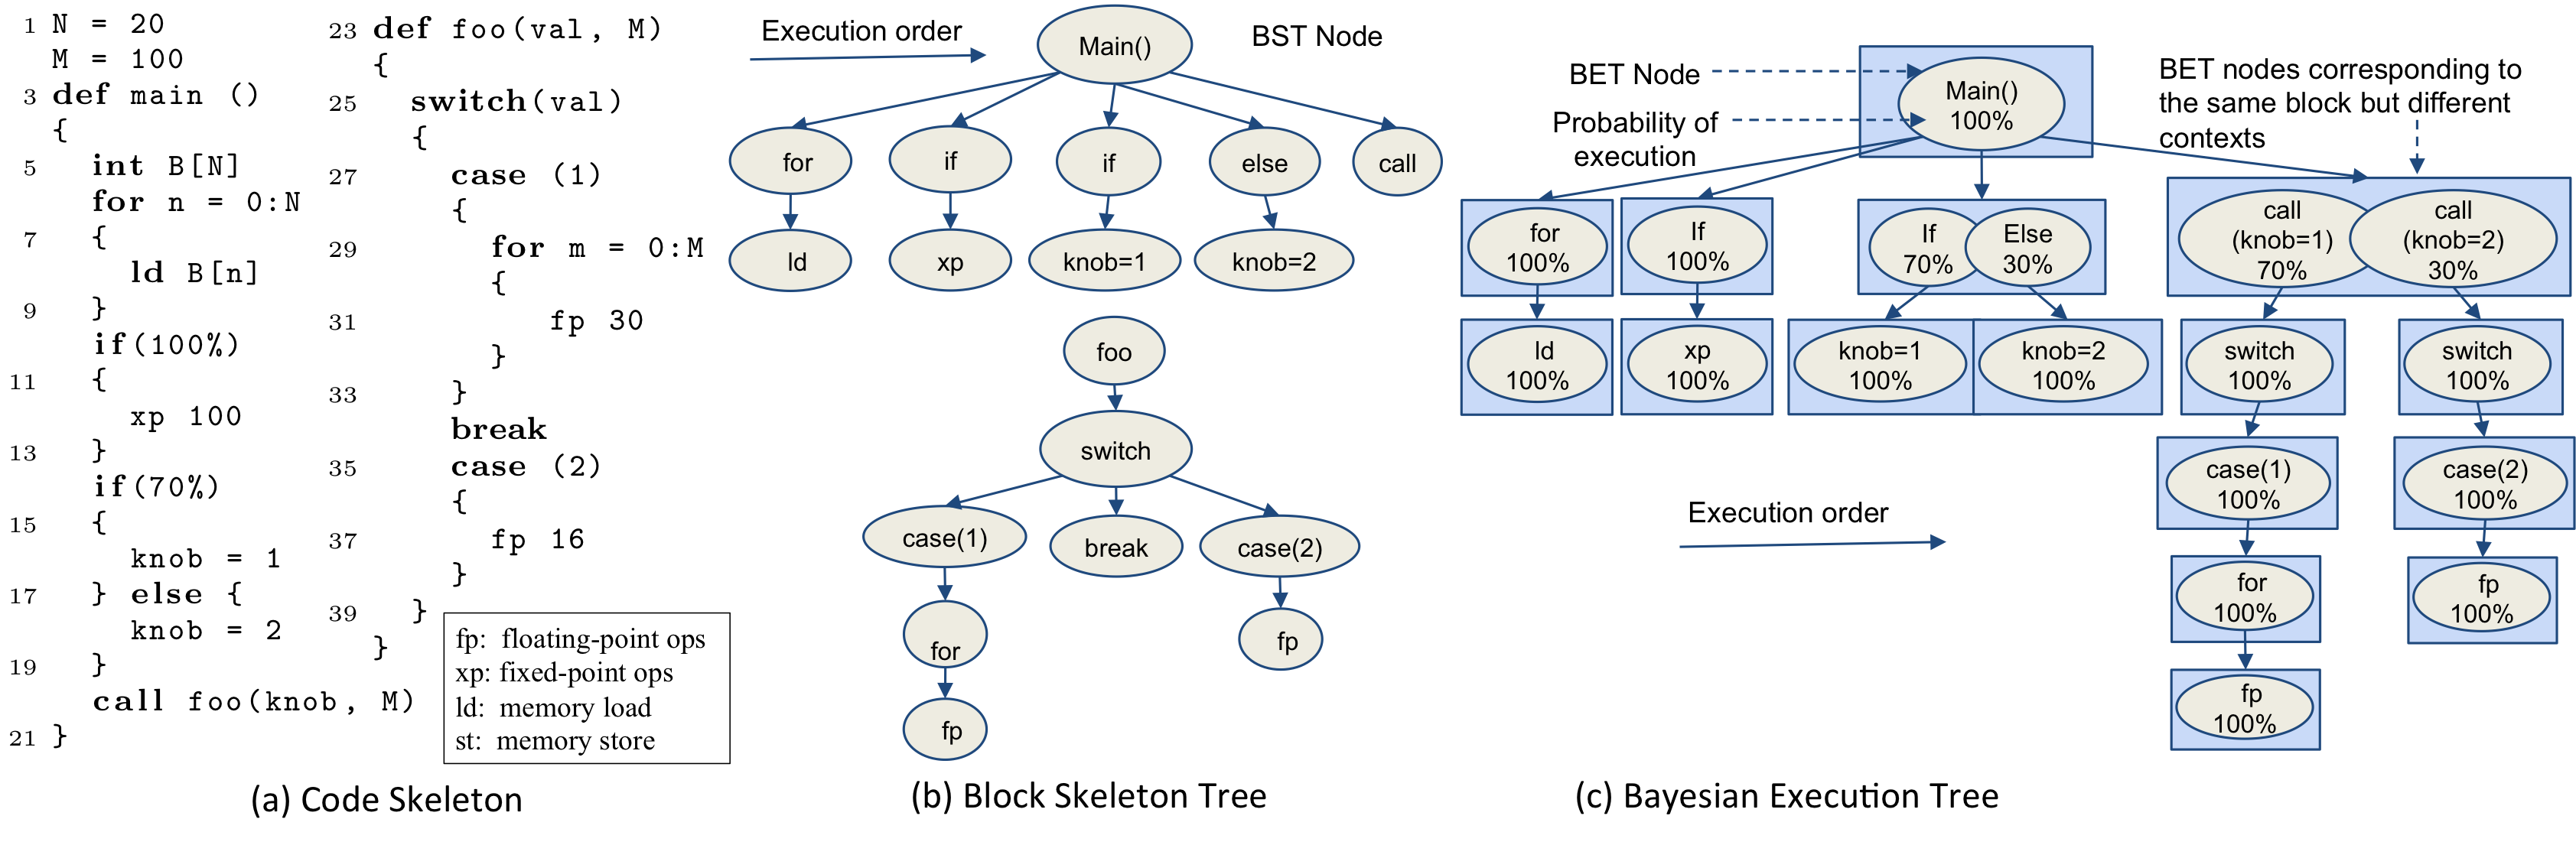
\includegraphics[width=0.98\textwidth]{fig/bstbet.png}
%\caption{An example code skeleton, and its corresponding block skeleton tree and bayesian execution tree.}
%\label{fig:bstbet}
%\end{center}
%\end{figure*}

%\ASPLOS{
%\subsection{Generating Code Skeletons}
%
%%While code skeletons are originally proposed to autotune kernels and are coded manually,
%Within the original SKOPE framework~\cite{skope},
%code skeletons were manually generated from an existing application.
%Using the
%ROSE compiler framework~\cite{rose}, we have developed an application analysis engine
%to automatically convert Fortran or C code into code skeletons.
%It is composed of two components: a source-to-source translator
%and a branch profiler.
%The source-to-source translator statically characterizes
%the instruction mix, array accesses, and control flow structures.
%The branch profiler profiles a program on a local machine using gcov~\cite{gcov}
%to obtain branch outcome statistics such as
%the iteration counts of loops with uncertain boundaries (e.g., {\tt while} loops)
%and fall-through probabilities for data-dependent branches.
%Such information is hardware independent and is encoded as expressions of the input data,
%%The resulting information is incorporated into the code skeleton.
%% jichi 12/16/2013
%% IPDPS review#2
%% - A comment in the paper on the issue of input sets, as described above would be very helpful.
%% => address
%\IPDPSREVIEW{
%specifically
%%The skeleton itself only contains the information in the source code.
%%It does not have input data set.
%%The information of the input data is summarized by hint files,
%the input data sizes and distribution of values, which are summarized in a  {\em hint file}
%%manually specified
%provided by the developers.
%}%\IPDPSREVIEW
%Currently, the code skeleton analysis engine
%only supports programs with regular data structures such as arrays, which
%are the most widely used in scientific application.
%Accommodating more complex pointer-based structures remains future work.
%%Due to space limitations, we focus the rest of the paper on
%In the rest of the paper, we focus on
%execution flow modeling and performance analysis using the generated code skeleton.
%
%% jichi 12/16/2013
%% IPDPS review#2
%% Add an outline of the assumption. For example, in Section 3B, it is mentioned that only "regular data structures" are supported.
%% => deficiency of pointers
%\IPDPSREVIEW{
%Our current skeleton generation process is domain specific,  with a focus on
%scientific workload and array operations. As a first-order approximation,
%our static analysis does not
%take into account issues associated with the limited number of registers, instruction
%level dependences, and potential compiler optimizations to manage these issues.
%% Our skeleton generation process is based on several assumptions for the applications to model.
%%\begin{itemize}
%%\item We assume there are no complex pointer-based data structures in the source code.
%%Accommodating more complex pointer-based structures remains future work.
%%\item We assume there are infinite number of registers, so that the scalar variables will not spill.
%%So, scalar variables will not produce load and stores,
%%  which only come from array accesses.
%%\item The generation process is ignorant of compiler optimizations.
%%Our generated skeleton is a direct model of the original source code.
%%It does have the optimizations applied by compilers.
%%\end{itemize}
%}%\IPDPSREVIEW
%
%}%\ASPLOS

%\subsection{Communication Cost Projection}
%
%To analytically estimate the runtime for MPI applications,
%a communication model is needed for projecting performance of MPI communication offline.
%Based on the LogP theory,
%I developed a communication model
%to estimate the communication time for point-to-point or collective communication
%given the message size and number of nodes.
%The model could be formulated by the following equation:
%\begin{equation}
%runtime = F_{mpi\_type}(message\_size; node\_number)
%\end{equation}
%It takes the type of the MPI communication,
%number of nodes, and data transfered,
%and output the estimated communication time
%excluding the balancing time.
%The type of the MPI communication including point-to-point send/recv and collective functions.
%In my framework, the communication model is created by profiling kernel MPI benchmarks over the target hardware.
%
%The following subsections will discuss the communication model, the profiled kernel benchmarks,
%and the statistical analysis for constructing the model.
%
%\subsection{Communication cost and message size}
%The communication cost can be estimated using LogGP model from
%the process number ($p$),
%message size ($n$),
%and platform-specific constant parameters ($alpha$, $beta$, $gamma$, \ldots).
%In my framework, MPICH is the MPI runtime environment on the target machines.
%In MPICH 3.1,
%the communication cost is usually proportional to the message size for both point-to-point and collective communication.
%
%\subsubsection{MPI\_Send and MPI\_Recv}
%According to the LogGP model, the point-to-point communication can be modeled as a linear equation for both small and large message sizes:
%\begin{equation}
%cost_{p2p} = alpha + n\cdot beta
%\end{equation}
%
%\subsubsection{MPI\_Alltoall}
%In MPICH 3.1, the communication algorithm is different for small and large message sizes.
%\begin{equation}
%cost_{a2a}|_{n<threshold} = log P\cdot alpha + (n/2)\cdot log P\cdot beta
%\end{equation}
%\begin{equation}
%cost_{a2a}|_{n>threshold} = (p-1)\cdot alpha + n\cdot beta
%\end{equation}
%In each case, the overall cost is proportional to the message size $n$.
%
%\subsubsection{MPI\_Alltoallv}
%In MPICH 3.1, the Alltoallv is implemented as decoupled non-blocking send and receives.
%So, the communication cost should be proportional to the overall message size.
%
%\subsubsection{MPI\_Bcast and MPI\_Reduce}
%The cost for broadcast and reduce in MPICH 3.1 is as follows where the cost is proportional to the message size $n$.
%\begin{equation}
%cost_{bcast} = log P\cdot alpha + n\cdot log P\cdot beta
%\end{equation}
%\begin{equation}
%cost_{reduce} = log P\cdot alpha + n\cdot log P\cdot beta + n\cdot log P\cdot gamma
%\end{equation}
%
%%  Cost = lgp.alpha + n.((p-1)/p).beta
%%\subsubsection{MPI\_Gather}
%
%\subsection{Analytic communication model}
%Given the fact that the communication cost is proportional to the message size
%but could the communication algorithm could change for small or large message size,
%different MPI communication model can be generalized
%as a broken-line linear equation:
%\begin{equation}
%cost(n;p) = \sum_i(alpha_{i,p} + n\cdot beta_{i,p})|_{threshold_i<n<threshold_{i+1}}
%\end{equation}
%Given fixed processor number $p$, the communication cost is a linear equation of
%message size $n$ within a pair of message size thresholds.
%The parameters $alpha$ and $beta$ are determined by the processor number and the range of the thresholds
%and runtime-dependent on the target platform.
